\documentclass[handout]{beamer}
\usepackage{framed}
%to include graphics
\usepackage{graphicx}
%to include code
\usepackage{listings}
\usepackage{courier}
%to include hyperlinks
\usepackage{hyperref}
\usepackage{caption}
\usepackage{pifont}
%used for amsfonts
\usepackage{amsmath}
%used for mathscr
\usepackage{mathrsfs}
%used for indicator function (mathbbm)
\usepackage{dsfont}
%no page numbering
%\usepackage{nopageno}
%used for aligning graphics
%\usepackage{adjustbox}

\lstset{
         basicstyle=\tiny\ttfamily, 	% Standardschrift
         %numbers=left,     			% Ort der Zeilennummern
         numberstyle=\tiny,          % Stil der Zeilennummern
         %stepnumber=2,              % Abstand zwischen den Zeilennummern
         numbersep=5pt,              % Abstand der Nummern zum Text
         tabsize=2,                  % Groesse von Tabs
         extendedchars=true,         %
         breaklines=true,            % Zeilen werden Umgebrochen
         keywordstyle=\color{red},
    		frame=b,         
 %        keywordstyle=[1]\textbf,    % Stil der Keywords
 %        keywordstyle=[2]\textbf,    %
 %        keywordstyle=[3]\textbf,    %
 %        keywordstyle=[4]\textbf,   \sqrt{\sqrt{}} %
         stringstyle=\color{white}\ttfamily, % Farbe der String
         showspaces=false,           % Leerzeichen anzeigen ?
         showtabs=false,             % Tabs anzeigen ?
         xleftmargin=17pt,
         framexleftmargin=17pt,
         framexrightmargin=5pt,
         framexbottommargin=4pt,
         %backgroundcolor=\color{lightgray},
         showstringspaces=false      % Leerzeichen in Strings anzeigen ?        
 }
 
\linespread{1.3}


\DeclareCaptionFont{white}{\color{white}}
\DeclareCaptionFormat{listing}{\colorbox[cmyk]{0.43, 0.35, 0.35,0.01}{\parbox{\textwidth}{\hspace{15pt}#1#2#3}}}
\captionsetup[lstlisting]{format=listing,labelfont=white,textfont=white, singlelinecheck=false, margin=0pt, font={bf,footnotesize}}


%for beamer theme
\usetheme[pageofpages=of,% String used between the current page and the
                         % total page count.
          bullet=circle,% Use circles instead of squares for bullets.
          titleline=true,% Show a line below the frame title.
          alternativetitlepage=true,% Use the fancy title page.
          ]{Torino}

\setbeamercovered{invisible}          
\setbeamertemplate{section page}
{
	\huge{\insertsection}
	 \textcolor{chameleongreen3}{\hrule height 1pt} 	
  	\vspace{0px}
}  

\newcommand{\hiddencell}[2]{\action<#1->{#2}}
% first argument: slide number to appear from, second argument: content of cell        

%-----------------------------------------------------------
%-----------------------------------------------------------
%-----------------------------------------------------------
%-----------------------------------------------------------

\author[Johanning]{Simon Johanning}
\title{Early gene regulation of osteogenesis in embryonic stem cells}
\institute{Institut f\"ur Mathematik und Informatik der Universit\"at Leipzig}

%\pagestyle{plain}
\AtBeginSection{\frame{\sectionpage}}

\begin{document}	
\watermarkoff

\begin{frame}[t,plain]
	\titlepage
\end{frame}

\section{Motivation}

\begin{frame}{Kontext}
\begin{itemize}
	\item Signal pathways und Ver\"anderung in Genexpression von Stammzellendifferentiation von M\"ausen (mES) nicht gut charakterisiert
	\pause
	\item Differenzierung in pluripotente Zellen in Knochengewebe essentiell f\"ur therapeutische Anwendungen (insbesondere tissue engineering)
	\pause
	\item Wachstumsfaktoren sind potente Regulatoren von Differenzierung 	von M\"ausen
\end{itemize}
\end{frame}

\begin{frame}{Wachstumsfaktoren}
\begin{itemize}
	\item Wichtige Wachstumsfaktoren Osteogenese: BMP2 (\emph{Bone Morphogenetic Protein 2}) und TGF$\beta$1 (\emph{Transforming Growth Factor $\beta$1})
	\pause
	\item BMP2: positiver Regulator in Osteogenese
	\pause
	\item TGF$\beta$1: negativer Regulator in O.; hohe Konzentration in Knochen und Knorpelgewebe
	\pause
	\item Aber: Manche Studien sehen TGF$\beta$1 als pro-osteogenisch, manche als kontra-osteogenisch
	\pause
	\\ Spielt Schl\"usselrolle in ihrer Regulation
	\pause
	\\ Es gibt viele Studien, die suggerieren, dass TGF$\beta$1 pro-osteogen ist
\end{itemize}
\end{frame}

\begin{frame}{Wachstumsfaktoren}
\begin{itemize}
	\item Rolle von TGF$\beta$1 in Osteogenese h\"angt von Zelltyp und lokaler Umgebung ab
	\pause
	\item TGF$\beta$1 alleine kann keine \emph{de novo} Osteogenese initiieren
	\pause
	\item wenige \emph{in vitro}-Studien, die sowohl TGF$\beta$1 als auch BMP2 untersuchen
	\pause
	\item $\rightarrow$ Motivation f\"ur diese Studie
\end{itemize}
\end{frame}

\begin{frame}{Gene}
\begin{itemize}
	\item Runx2 wesentliches regulatorisches Gen (Transkiptionsfaktor) in Osteoblasten
	\pause
	\\ Wichtig f\"ur (down-stream) Expression vieler osteogenetischen Gene
	\pause
	\item Bekannt, dass von BPM2 und TGF$\beta$1 reguliert
	\pause
	\item Ebenso von Genen Dlx5 und Msx2, welche beide von BPM2 und TGF$\beta$1 stimuliert werden
\end{itemize}
\end{frame}

\begin{frame}{Gene}
\begin{itemize}
	\item Dlx5 von BMP2 allein stimuliert
	\pause
	\item Dlx5 stimuliert Runx2
	\pause
	\item Msx2 wird oft als negativer Regulator von Runx2 gesehen (bindet an Runx2-Promoter ohne Expression zu induzieren)
	\pause
	\\ Aber: Rolle nicht so klar; Manche Studien: Msx2 supprimiert, manche kein Effekt, manche pro-osteogenetisch unabh\"angig von Runx2
\end{itemize}
\end{frame}

\begin{frame}{Genregulationsnetzwerke}
\begin{itemize}
	\item Signal- und Regulationsnetzwerke, die Interaktion zwischen BMP2 und TGF$\beta$1 regeln, sind nicht bekannt
	\pause
	\item Kandidaten f\"ur Netzwerke: Dlx5 und Msx2, da diese um Runx2-Promoter konkurrieren
\end{itemize}
\end{frame}

\begin{frame}{Motivation mathematische Modelle}
\begin{itemize}
	\item Schwierig Unterschiede zwischen Versuchsgruppen und verschiedenen Zeiten zu analysieren
	\pause
	\\ $\rightarrow$ problematisch analytisch Beziehungen zwischen Dlx5, Msx2 und Runx2
	\\ $\rightarrow$ mathematische Modellierung der Netzwerke und Vergleich mit experimentellen Daten
\end{itemize}
\end{frame}

\section{Mathematische Modellierung}

\begin{frame}{Boolsche Modelle}
\begin{itemize}
	\item Rigorose Repr\"asentation qualitativen biologischen Wissens
	\pause
	\item Komponenten (\emph{Spezies}) haben diskrete Zust\"ande; oftmals bin\"ar: \emph{An/Aus}
	\pause
	\item Repr\"asentation als Graphen: Gene/Faktoren als Knoten, Kanten als Interkationen (aktivierend/inhibierend)
	\pause
	\item Diskrete Zeit: Zustand(t+1) h\"angt von Zust\"anden(t) ab
	\pause
	\item stabile steady-states: Zellph\"anotypen, die mit experimentellen Daten verglichen werden k\"onnen
	\pause
	\item Auch wenn grob, k\"onnen BM das qualitative Verhalten biologischer Systeme recht gut reproduzieren
\end{itemize}
\end{frame}

\begin{frame}{Boolsche Modelle: Beschr\"ankungen}
\begin{itemize}
	\item K\"onnen weder kontinuierliche Konzentrationslevel noch realistische Zeitskalen abbilden
	\pause
	\\ $\Rightarrow$ K\"onnen quantitative (biologische) Experimente weder erkl\"aren noch vorhersagen
	\pause (zunehmend wichtig in systems biology)
	\\ \pause $\rightarrow$ \"Ubergang zu Differentialgleichungssystemen: HillCube model / odefy
\end{itemize}
\end{frame}

\begin{frame}{odefy}
\begin{itemize}
	\item Erlauben detailliertere und quantitative Charakterisierung der Genregulationsnetzwerke
	\pause
	\item Einfach Eingangskonzentrationen und Parameter zu modellieren
	\pause
	\item stabile steady-states in ODEs: Zellph\"anotypen
\end{itemize}
\end{frame}

\begin{frame}{odefy}
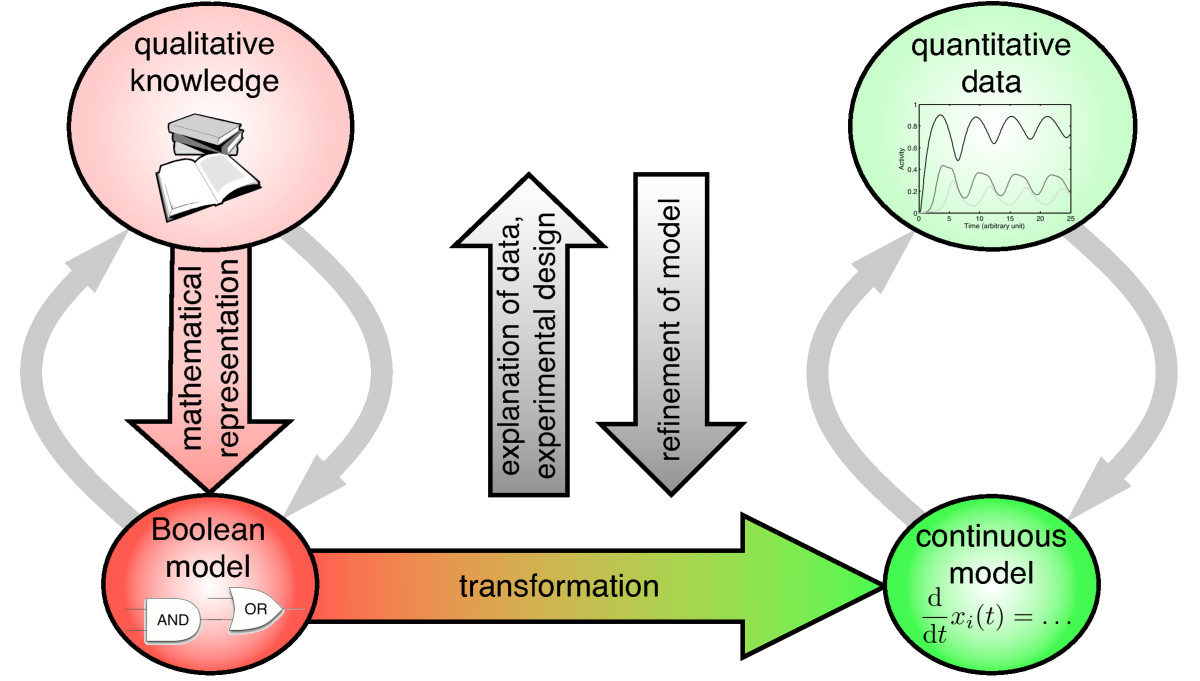
\includegraphics[scale=0.8]{odefy.jpg}
\end{frame}

\begin{frame}{Generalisierung boolsches Modell}
\begin{itemize}
	\item Ph\"anomenologische Beschreibung von Prozessen
	\pause
	\item Lassen oft Einflussfaktoren und Zwischenschritte aus
	\pause
	\\ $\rightarrow$ Kontinuierliche Modelle sind ebenso ph\"anomenologisch
	\pause
	\item Top-down Methode f\"ur Netwerke mit inkompletten Wissen, wo kinetische Modellierung unpraktisch ist
	\pause
	\item Kontinuierliches Modell kann Verhalten des Booleschen Modells reproduzieren, aber auch verschiedene Zeitskalen der Interaktion modellierung
	\pause
	\\ $\rightarrow$ Generalisierung des boolschen Modells (mehr dynamische Eigenschaften).
\end{itemize}
\end{frame}

\begin{frame}{Formale Darstellung boolsches Modell}
\begin{itemize}
	\item $N$ Spezies $X_{1}, X_{2},..., X_{N}$ mit $x_{i} \in \{0,1\}$
	\pause
	\item F\"ur jede Spezies: Menge von Spezies, die $x_{i}$ beeinflussen: $R_{i} := \{X_{i_{1}}, ..., X_{i_{2}}, X_{i_{N}}\} \subset \{X_{i_{1}},...,X_{i_{N}}\}$
	\pause
	, \\ sowie eine Aktualisierungsfunktion $B_{i}: \{0,1\}^{N_{i}} \to \{0,1\}$ f\"ur jede Kombination von $(x_{i_{1}}, ..., x_{i_{2}}, x_{i_{N_{i}}}) \in \{0,1\}^{N_{i}}$
	\pause
	\item Betrachte $B_{i}$ auf (Hyper-)Einheitsw\"urfel: Knoten $(\xi{i_{1}}, ..., \xi{i_{2}}, \xi{i_{N_{i}}}) \in \{0,1\}^{N_{i}}$ entspricht $(\bigwedge_{ij | \xi{ij} = 1} x_{ij}) \wedge (\bigwedge_{ij | \xi{ij} = 0} \neg x_{ij}) $
\end{itemize}
\end{frame}

\begin{frame}{Formale Darstellung boolsches Modell}
\begin{itemize}
	\item sum-of-product Repr\"asentation: $B(x_{i_{1}}, ..., x_{i_{2}}, x_{i_{N_{i}}}) = \bigvee_{(\xi_{i_{1}}, ..., \xi_{i_{2}}, \xi_{i_{N_{i}}}) | B_{i}(\xi_{i_{1}}, ..., \xi_{i_{2}}, \xi_{i_{N_{i}}})=1 } [(\bigwedge_{ij | \xi{ij} = 1} x_{ij}) \wedge (\bigwedge_{ij | \xi{ij} = 0} \neg x_{ij})] $
	\pause
	\item Nun ersetzen von $x_{i} \in \{0,1\}$ durch $\overline{x_{i}} \in [0,1] \rightarrow \overline{B_{i}}: [0,1]^{n} \to [0,1]$: kontinuierliche homologe von $B_{i}$
	\pause
	\item Normalisierte HillCubes: $\overline{B}^{H}_{n_{i}}(\overline{x_{1}}, \overline{x_{2}},...,\overline{x_{n}}) := \overline{B}^{I}_{i}(\frac{f_{i_{1}}(\overline{x_{i_{1}}})}{f_{i_{1}}(1)},\frac{f_{i_{2}}(\overline{x_{i_{2}}})}{f_{i_{2}}(2)},...,\frac{f_{i_{n}}(\overline{x_{i_{n}}})}{f_{i_{n}}(n)})$
\end{itemize}
\end{frame}

\begin{frame}{HillCubes}
\begin{itemize}
	\item $\overline{B_{i}}^{I}$: lineare Interpolation von $B_{i}$ mittels multivariater polynomialer Interpolation: BooleCubes. 
	\pause
	$\overline{B_{i}}^{I}$ affin multilinear: $ 1 \leq j \leq N_{i}, \overline{x}_{ik} \text{ fix }: \exists a,b \in \mathbb{R}: \overline{B_{i}}^{I}(\overline{x}_{i1},\overline{x}_{i2},...,\overline{x}_{iN_{i}}) = a + b \overline{x}_{ij}$
	\pause
	\item f: Hill-Funktionen: $f(\overline{x}) = \frac{\overline{x}^{n}}{\overline{x}^{n} + k^{n}}$
	\pause
	\item Sigmoide Funktionen mit
	\\ n: Anstieg der Funktion: Kooperativit\"at der Interaktion
	\\ k: Schwellenwert des Boolschen Modelles (Halbmaximalit\"at von f)
	\pause
	\item $\frac{f_{i_{\ell}}(\overline{x_{i_{\ell}}})}{f_{i_{\ell}}(\ell)}$: Normalisierung, sodass $f(\zeta)=1$ erreicht wird
\end{itemize}
\end{frame}

\begin{frame}{Eigenschaften HillCubes}
\begin{itemize}
	\item  $\overline{B} := \overline{B}^{H}_{n_{i}}(\overline{x_{1}}, \overline{x_{2}},...,\overline{x_{n}}) := \overline{B}^{I}_{i}(\frac{f_{i_{1}}(\overline{x_{i_{1}}})}{f_{i_{1}}(1)},\frac{f_{i_{2}}(\overline{x_{i_{2}}})}{f_{i_{2}}(2)},...,\frac{f_{i_{n}}(\overline{x_{i_{n}}})}{f_{i_{n}}(n)})$ ist perfektes Homolog von $B_{i}$
	\pause
	\item steady-states von Boolschen Modellen \"ubertragen sich
	\pause
	\item HillCubes stimmen auf Knoten mit BoolCubes \"uberein
	\pause
	\item Haben 'sch\"one' analytische Eigenschaften (bspw. Stetigkeit)
	\pause
	\item Eindeutige minimale L\"osung innerhalb Funktionenklasse
\end{itemize}
\end{frame}

\begin{frame}{Konstruktion kontinuierliches Modell}
\begin{itemize}
	\item Option 1 (zeitdiskretes Modell): $\overline{x}_{i}(t+1) = \overline{B}_{i}(\overline{x}_{i_{1}}(t),\overline{x}_{i_{2}}(t),...,\overline{x}_{i_{N_{i}}}(t))$
	\pause
	\\ Nachteil: Unsteitigkeit l\"asst analytische Methoden nicht zu
	\pause
	\item Option 2 (zeitkontinuierliches Modell): Annahme: $\overline{B_{i}}$ ist Produktionsrate von $\overline{x_{i}}$, Abbau mit Rate $\overline{x_{i}}$:
	\pause
	\\ Differentialgleichung $\dot{\overline{x_{i}}} = \frac{1}{\tau_{i}} (\overline{B_{i}}(\overline{x}_{i_{1}},\overline{x}_{i_{2}},...,\overline{x}_{i_{N_{i}}}) - \overline{x_{i}})$
	\\ mit $\tau_{i}$ Lebensdauer der Spezies $X_{i}$
\end{itemize}
\end{frame}

\section{Modellierung paper}

\begin{frame}{Versuchsaufbau}
\begin{itemize}
	\item Beobachung von Dlx5, Msx2 und Runx2 embrionischen Stammzellen (Maus) \"uber Zeitraum von 48 Stunden
	\pause
	\item Kontrollkondition: Stammzellen ohne Zugabe von Wachstumsfaktoren
	\pause
	\item Dlx5: Nach 24 Stunden signifikant gesteigerte Expression mit BMP2 und BMP2/TGF$\beta$1 (Kombination st\"arkerer Effekt)
	\pause
	\item Msx2: TGF$\beta$1 deutlich reduzierte Expression (ab 16 Stunden). 
	\pause
	\\ BMP2: h\"ohere Expression als TGF$\beta$1 und BMP2/TGF$\beta$1
	\item Runx2: Erh\"ohte Expression sowohl mit TGF$\beta$1 als auch BMP2, aber nicht in Kombination
\end{itemize}
\end{frame}

\begin{frame}{Resultate Experiment}
\begin{center}
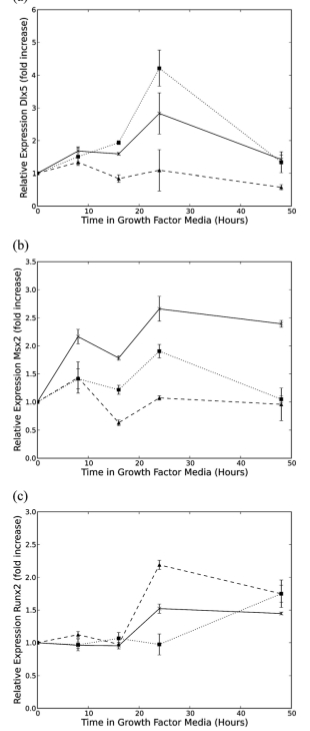
\includegraphics[scale=0.25, center]{expression_experiment.jpg}
\end{center}
\end{frame}

\begin{frame}{Setup mathematisches Modell}
Modellierung Genregulationsnetzwerk nach bestehenden Studien
	\pause
	: 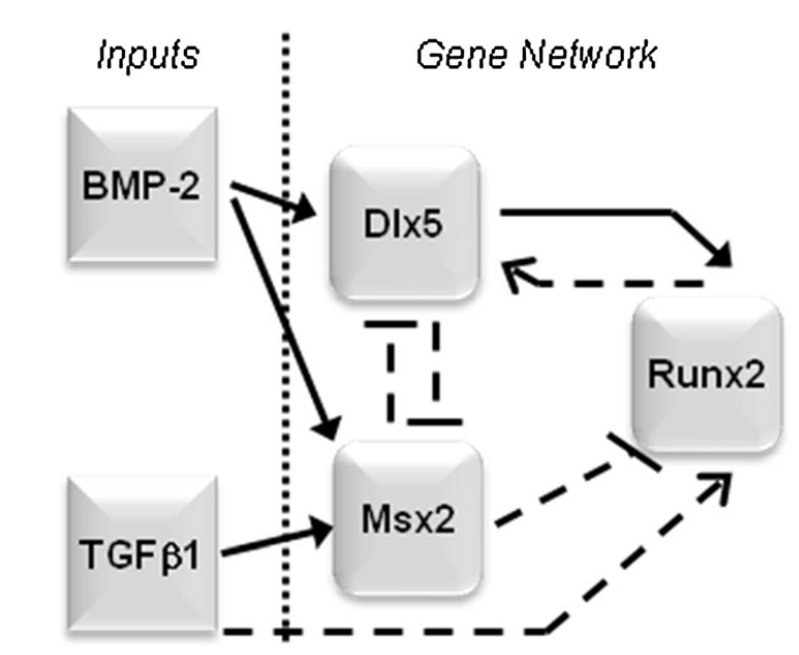
\includegraphics[scale=0.22]{regulatory_network.jpg}
\end{frame}

\begin{frame}{Setup mathematisches Modell II}
\begin{itemize}
	\item Konstruktion boolscher Modelle, die konsistent mit Beobachungen der Expressionsprofile sind ($t \in \{0,24\}$); 
	\pause
	\\ \emph{An} falls signifikanter Unterschied zu t=0, sonst \emph{Off} (da mRNA niedrig in mES-Zellen)
	\pause
	\item Modelle, die zu experimentellen Daten passen: Regulation von Dlx5 durch Runx2 unklar
\end{itemize}
\end{frame}

\begin{frame}
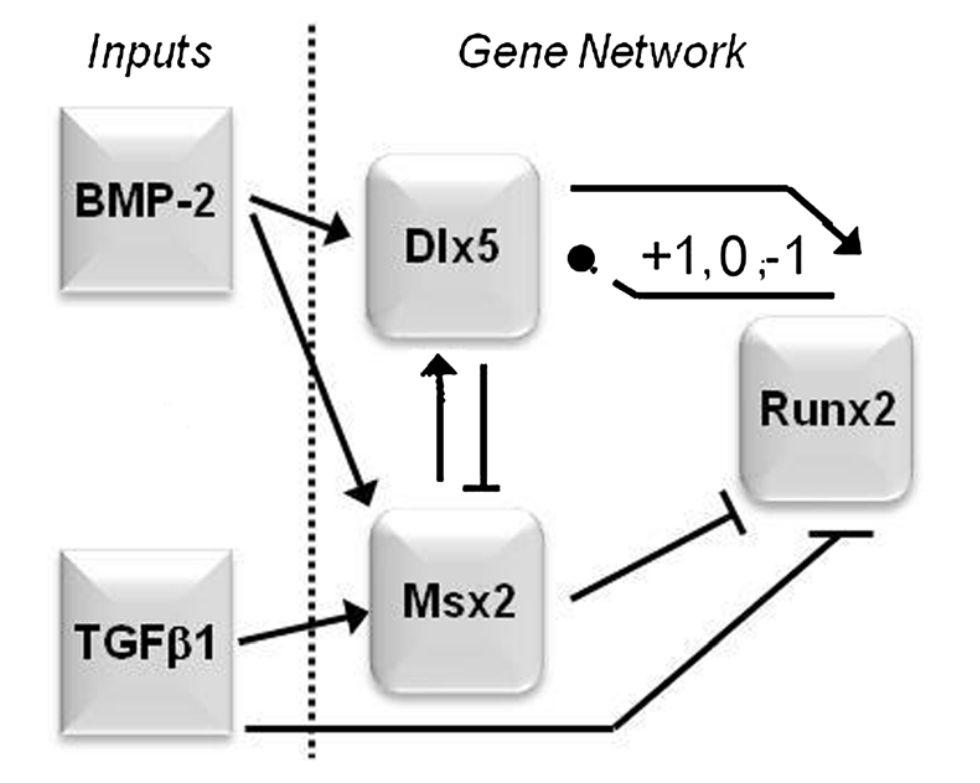
\includegraphics[scale=0.24]{regulatory_network_results.jpg}
\end{frame}

\begin{frame}{Setup mathematisches Modell III}
\begin{itemize}
	\item Transformation in ODE mittels \emph{HillCube}-Methode
	\pause
	\item Fitten der Differentialgleichungen mittels experimenteller Daten ($t \in \{0,8,16,24\}$) mittels Parametersch\"atzung mit \emph{EcsPy} (Python-Modul)
\end{itemize}
\end{frame}

\begin{frame}{Unter- / \"Uberexpression}
\begin{itemize}
	\item Untersuchung des Einflusses von Runx2 auf Dlx5:
	\pause
	\\ Positive Regulation: Gesteigerte Expression in TGF$\beta$1 und Kontrollmedium, verringerte Expression von Msx2 in TGF$\beta$1 
	\item Festhalten des Expressionslevel an 0 (Unterexpression), 1 (\"Uberexpression): 
\end{itemize}
\end{frame}


\section{Ergebnis}

\begin{frame}{Ergebnis}
\begin{itemize}
	\item Simulationen: Boolsche Modelle ergeben oszillierende Ergebnisse in TGF$\beta$1, wobei ODE-Modelle dies nur ergeben, wenn Runx2 Dlx5 negativ reguliert
	\pause (intuitiv sinnvoll, da Oszillationen nur auftreten, wenn alle Transkriptionsfaktoren sowohl hoch- als auch heruntergeregelt werden k\"onnen, und TGF$\beta$1 sowohl als positiver wie negativer Regulator Osteogenese gesehen wird)
	\pause
	\item Nur ein Modell zeigt mit Experiment konsistentes Verhalten
	\\ $\rightarrow$ Alle anderen Modelle verworfen
	\pause
	\item Modell bildet weiterhin das Verhalten der Transkiptionsfaktoren ab (Runx2 beginnt nach Dlx5 und Msx2)
\end{itemize}
\end{frame}

\begin{frame}
\begin{center}
	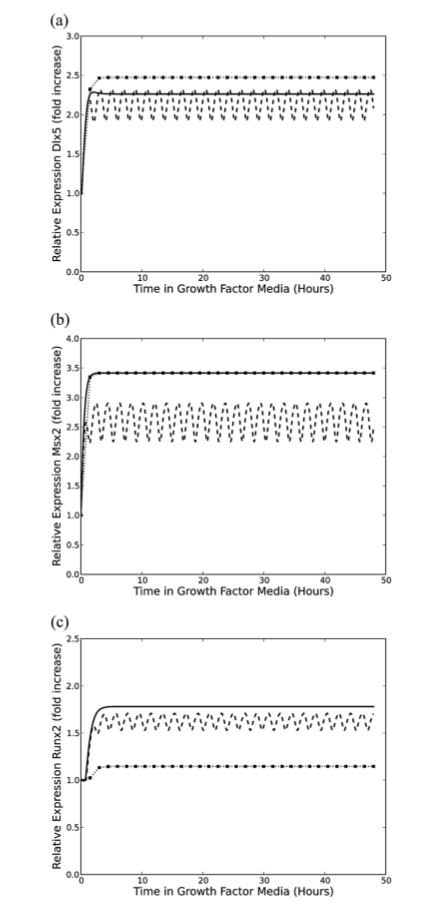
\includegraphics[scale=0.26]{oscillations.jpg}
\end{center}
\end{frame}

\begin{frame}{Ergebnis}
\begin{itemize}
	\item Erh\"ohte Expression von Runx2 in BMP2-Medium wird von Ver\"anderung in Dlx5-Expression beeinflusst 
	\pause
	\\ Diese wiederum wird durch erh\"ohte BMP2-Konzentration oder BMP2-Msx2-Mechanismus erreicht
	\pause
	\item Erh\"ohte Expression von Runx2 in TGF$\beta$1 legt nahe, dass dieses durch Msx2-Stimulation von Dlx5 bedingt ist
	\pause
	\item Weiterhin funktioniert Dlx5 als negativer Regulator von Msx2 (und somit indirekt hemmend auf Zellproliferation)
	\pause
	\item Verhalten im Bezug auf TFG$\beta$1 und Einfluss von Msx2 in dieser Studie das erste Mal aufgezeigt
\end{itemize}
\end{frame}

\section{Kritik}

\section{Praktikumsarbeit}

\end{document}